\chapter{Introduction}
  \section{Drug Discovery Today}
    New drug development is a lengthy and costly process, and a recent study reported an average cost of $\sim$ 2558 million US dollars in developing a new drug \cite{dimasi2016innovation}. Part of the reason of the high cost is due to the high failure rate of preclinical drug candidates, which is largely caused by lack of efficacy of these candidates; this indicates that the wrong target is pursued \cite{shih2018drug}. Computational drug repositioning and target discovery may serve as a new way to shorten the process of drug development, due to the lower cost and more established safety profile of existing drugs \cite{dudley2011exploiting}. A number of in silico approaches have been developed for drug repositioning and target discovery and are reviewed elsewhere \cite{hodos2016silico,vanhaelen2017design,kandoi2015prediction}. With the rapid rise of machine learning (ML) technologies in the past decade, there has been a rising interest in applying ML methods in drug repositioning or target discovery. 

    Machine learning refers to a vast number of methods for computers to "learn" and gain insight into data without human interference. These methods are classified into two categories: supervised and unsupervised. Supervised machine learning methods are models for prediction or estimation based on one or more inputs. They are called supervised methods, as their learning is "supervised" by known output values. On the other hand, unsupervised machine learning methods can be used to detect relationship or patterns underlying "unlabeled" data. Here we focus on supervised learning methods for classification, since in most cases studies related to drug discovery using ML are the application of classification algorithms. One approach to drug repurposing is to employ drug expression profiles as predictors (i.e., features) to predict a drug’s treatment potential. The outcome variable can be the drug category (e.g., whether it is a cardiovascular or anticancer agent) or whether the drug is indicated for a particular disorder (e.g., whether the drug is indicated for diabetes). In the former case, drugs that are classified into categories other than its own indications may be considered for repositioning. In the latter case, drugs with high predicted probabilities but not indicated for the disorder may serve as candidates for repositioning. Additionally, we may also interested in whether the expression profile induced by genetic perturbation (e.g. over-expression or knock down) showed similar pattern to expression profiles of drugs considered as treatments for specific disease, since in this case the perturbed gene can be considered as promising target for the disease. Note that indications for drugs can easily be obtained from publicly available resources such as the Anatomical Therapeutic Chemical (ATC) Classification System \cite{wei2013development}. An important advantage is that ML algorithms are abundant and in rapid development, and any existing or new algorithms can be applied without much modification.

    With the growth of availability of biomedical data, especially “omics”, computational methods can offer a fast, cost-efficient and systematic way to priority promising drug target and drug repurposing candidates for various diseases. The approach has several advantages. Specifically, finding new indications for existing drugs, an approach known as drug repositioning or repurposing, can serve as a useful strategy to shorten the development cycle. Repurposed drugs can be brought to the market in a much shorter time-frame and at lower costs. Meanwhile, computational drug target identification also can speed up the drug development by prioritizing the most promising drug target candidates in a short time, greatly reducing the time in seeking for potential drug targets. 

    There has been increasing interest in computational drug repositioning recently, in view of the rising cost of new drug development. Hodos et al. provided a comprehensive and updated review on drug repositioning \cite{hodos2016silico}, and G. Kandoi et. al. briefly reviewed applications of machine learning and system biology on discovery of target proteins \cite{kandoi2015prediction}. For the purpose of repositioning, similarity-based methods \cite{gottlieb2011predict,oh2014network,liu2015similarity,luo2016drug,napolitano2013drug,li2012new} usually were employed to explore repositioning opportunities, but as noted by Hodos et al., the dependence on data in the “nearby pharmacological space” might limit the ability to find medications with novel mechanisms of actions. Another related methodology is the network-based approach \cite{lotfi2018review}, which typically requires data on the relationship between drugs, genes and diseases as well as connections within each category (e.g. drug-drug similarities). It still constraints by the focus on a nearby pharmacological space and the choice of tuning parameters in network construction or inference is often ad hoc \cite{ferrero2017silico}. The present work is different in that we apply a broad framework for repositioning and we do not focus on one but many different kinds of learning methods. There is comparatively less reliance on known drug mechanisms or the "nearby pharmacological space" as we let the different algorithms "learn" the relationship between drugs, genes and disease in their own ways. We note that kernel-based ML methods such as support vector machine (SVM) are also based on some sort of similarity measures. A related work \cite{napolitano2013drug} have also examined SVM as a promising ML approach for drug repositioning and identified several interesting candidates. However, here our focus is different in that we considered a variety of other approaches and SVM is one of the methods which falls under the broader framework of ML for repositioning. 

    Although computational drug repositioning has attracted increased attention recently, few studies focus on psychiatric disorders, compared to other areas like oncology. Psychiatric disorders are leading causes of disability worldwide \cite{vigo2016estimating}, however there have been limited advances in the development of new pharmacological agents in the last two decades or so \cite{hyman2013psychiatric}. Development of new therapies is also limited by the difficulty of animal models to fully mimic human psychiatric conditions \cite{nestler2010animal}. Investment by drug companies has in general been declining \cite{hyman2013psychiatric} , and new approaches for drug discoveries are very much needed in this field. We will explore repositioning opportunities for schizophrenia along with depression and anxiety disorders. Here depression and anxiety disorders are analyzed together as they are highly clinically comorbid \cite{kessler2015anxious,otowa2016meta}, show significant genetic correlations\cite{otowa2016meta}, and share similar pharmacological treatments \cite{ballenger2000anxiety}.
    
    Meanwhile, we also have witnessed a rise in the interest of computational target discovery in recent years. G. Kandoi et. al. briefly reviewed applications of machine learning and system biology on discovery of target proteins \cite{kandoi2015prediction}. These studies explored different biological properties by machine learning methods to identify druggable targets \cite{bakheet2009properties,fauman2011structure,li2007prediction}. Biological features of human proteins like amino acid composition and amino acid property group composition were studied by a sequence-based prediction method to identify drug target proteins, and a comprehensive comparison of several machine learning methods was conducted \cite{kumari2015identification}. In another study, eight key properties of human drug target were extracted, and learned by support vector machine (SVM) to discover new targets; similar studies extracted simple physicochemical properties from known drug targets and explored the predictive power of these properties \cite{li2007prediction,emig2013drug}. Topological features of human protein–protein interaction network also were utilized by network based methods to identify potential drug targets \cite{li2015large}. In a recent study, gene-disease association data from Open Targets was explored by four different machine learning methods, including deep neuron networks, to find novel targets, and a large proportion of new targets identified were supported by previous literatures \cite{ferrero2017silico}. Dorothea Emig et. al. proposed an integrated network-based method to predict drug targets based on disease gene expression profiles and a high-quality interaction network, and some novel drug targets for scleroderma and other types of cancer were presented \cite{emig2013drug}. A most recent study proposed pairwise learning and joint learning methods constructed on chemically and genetically perturbed gene expression profiles, and outcome variable was defined as highly correlated pair given by the direct correlation calculation \cite{sawada2018predicting}. These studies aim to discover new targets by making use of structural attributes of proteins or properties of known targets, so targets with similar properties usually are identified, but drug targets with novel mechanisms are difficult to identify using this kind of approaches. Network based methods for target discovery, as mentioned previous, rely on known nearby targets to inference potential relationship, so they suffers the same drawback. 

    Even though repositioned drugs can be brought into market in a much shorter time, drug repositioning may not always be feasible (for example due to side-effects of existing drugs), and drug repositioning and target discovery can complement each other in drug development and pharmacological research. Additionally, in traditional drug development majority of drugs fail to complete the development process due to lack of efficacy, indicating that the wrong target is pursued \cite{shih2018drug}.Usually, a drug target is selected via analyzing how its function influences the disease. However, this process is time-consuming, because investigating a large number of potential targets is usually necessary for finding an ideal one \cite{phoebe2008identifying}. Computational methods can be utilized to hasten this process by prioritizing promising drug targets. 

  \section{Precision Medicine}
    Researchers have discovered hundreds of genes that harbor variations contributing to human illness. For example, genome wide association studies have identified 108 schizophrenia-associated genetic loci \cite{schizophrenia2014biological}. Genetic variability leads to patients response differently to dozens of treatments, and molecular causes of some diseases have been targeted in research. Direct-to-consumer (DTC) companies take advantage of DNA tests to provide genetic insights into personal traits and disease risks \cite{ng2009agenda}. The genetic testing can improve disease prevention \cite{heshka2008systematic}. Moreover, scientists have been beginning to utilize genetics or other molecular mechanisms to better predict patients' responses to targeted therapy \cite{hamburg2010path}. Particularly, there are successful examples in translation of cancer genomics into therapeutics and diagnostics. For instance, doctors recommend KRAS mutation testing for patients with colon or lung cancer before the initiation of  EGFR-targeted therapies; moreover, patients with RAS mutations are more likely to  benefit from pharmacological inhibition of the kinases MEK1 and 2 \cite{lievre2008kras}. Another clinically relevant question to individuals is how a risk factor will affect them individually. A more recent example is that the pandemic of coronavirus-19 has been attacking people globally, but only a minority of infected patients, including young adults, have respiratory failure \cite{ellinghaus2020genomewide}. There are numerous evidences to demonstrate the fact that different individuals response differently to the same risk factor. For example, not all obese persons develop cardiometabolic (CM) diseases though obesity is a well-known risk factor to the diseases \cite{neeland2018cardiovascular}. As another example, cigarette smoking is the top one risk factor for chronic obstructive pulmonary disease (COPD), but we still can find elder people with smoking habits do not develop COPD \cite{van2015we}. Conceptually, risk factors or treatments are equivalent, as risk factors can be considered as treatments with adverse effects. Exploration of the heterogeneity in subjects' outcomes in presence of risk factors is of great importance, since it allows us to offer tailored health management to each subjects. This enable us to offer personalized prevention or treatment strategies in a cost-effective way to benefit them the most. This is also the aim of "personalized medicine".

    The cost of genome sequencing have been decreased dramatically in the past decades. This increases the wide availability of "omics" data. On the advent of genomic ara, genetic data can be utilized to customize disease prevention and medical treatment.  Clinically, there are examples of success of personalized medicine, especially in cancer treatment. Chemotherapy medications such as trastuzumab and imatinib target specific cancers \cite{gambacorti2008part}. Despite all of these advances, only for a few diagnoses and treatment resort to patient's genetics information nowadays, end even if doctors can access to patients' genomes today, only a small percentage of the genome has been utilized \cite{yngvadottir2009promise}. Doctors still exercise 'one drug fits all' approach in the clinic. The key to 'personalized medicine' is to answer the most crucial concerns that how a RF or treatment will affect patients individually given their genetic and clinical information. The answer to this concern can advance our disease prevention and treatment. However, current researches on this issue largely focus on the average treatment effect of RFs in population rather than individualized treatment effects.
  
  \section{Supervised Machine Learning Methods}
    In this section we first define a general framework for supervised machine learning methods and then discuss several popular machine learning methods in detail. Let $X$ represent the real-valued input matrix (with dimension $n \times p$), where n and p denote the sample size and the number of features, respectively. $Y$ (with dimension $n$) denotes a random output vector. The subscript $i$ refers to the input or output of the $i$th observation. Our aim is to seek a function $f(x)$ for estimating $Y$ given the input $X$. A loss function $L$ is required to penalize the error made in the prediction. Thus, we choose $f$ that minimizes the following the equation \cite{friedman2001elements}:
    \begin{equation}
      \mathrm{EPE} (f) = \mathit{L}(f(X, Y)).
    \end{equation}
    Here EPE stands for the expected prediction error.

    \subsubsection{Linear Methods}
      The linear model is a simple and intuitive ML approach for regression and classification. In the case of biological systems, the true relationship underlying the data is often nonlinear. For example, in the current application, different genes may act in a complex and nonlinear manner to affect the potential of treatment. However, it can be regarded as a benchmark for the development of more sophisticated ML models. Basically, it assumes that the function $f$ we seek is linear:
      \begin{equation}
        f(X) = X \beta
      \end{equation}

      Here we assume the additional column with all 1 is added as the first column of $X$ for the ease of the equation representation; thus, the dimension of $X$ is $n \times (1 + p)$. $\beta$ is a vector of coefficients, with the first element denoting the intercept. When the output Y is real-valued, the typical loss function used is the squared error loss. This leads to a criterion for finding the optimal $\beta$, which minimizes the loss function below:
      \begin{equation}
        \mathrm{EPE} = (X \beta - Y)^T (X \beta - Y)
      \end{equation}

      However, the optimal coefficients $\beta$ chosen in a simple liner model as listed above may not yield the best predictive performance on new datasets, especially when the input is high-dimensional with low signal-to-noise ratio. One reason for this is that some noise may be learned by our model (i.e., the model "overfits"), leading to poor performance when applied in a new dataset. In the present application, transcriptome data is of high dimension, and it is reasonable to suspect that only a portion of the input genes may have significant effects on the potential of disease treatment.

      To overcome the above issue, regularized regression models can be used to do feature selection. In essence we penalize large values of $\beta$ to make the model less complex and less prone to overfitting, thus leading to prediction based on highly influential genes. The ridge penalty leads to coefficient shrinkage which can reduce the risks of model overfitting \cite{hoerl1970ridge}.

      However, some features may have little or no association with the output, and filtering out these features may make the interpretation easier and improve predictive performance. Another method known as LASSO (least absolute shrinkage and selection operator) can shrink coefficients down to zero \cite{tibshirani1996regression}, creating a sparse model with fewer features.

      In biomedical applications, some features (such as expression of genes in the same pathway) tend to be highly correlated. LASSO usually select one or several features from a group but ignore the others from the same group. Elastic net, a more advanced penalized regression method, may overcome this problem by combining ridge and LASSO penalties \cite{zou2005regularization}. The function we seek to minimize is as follows:
      \begin{equation}
        \mathrm{EPE} = (X \beta - Y)^T (X \beta - Y) + \lambda \bigg[ \alpha ||\beta||_{l_1} + \frac{1}{2} (1 - \alpha) ||\beta||_{l_2}\bigg]
      \end{equation}
      where $||\beta||_{l_1}$ denotes the L1 norm (i.e., sum of absolute values of $\beta$) and $||\beta||_{l_2}$ denotes the L2 norm (i.e., sum of the squared $\beta$) and $\lambda$ and $\alpha$ are tuning parameters. The elastic net regularization is a combination of L1 and L2 shrinkage. Ridge and LASSO regression are special cases of elastic net regression when $\alpha$ is 0 and 1, respectively.

      In regression, the output of linear model is a real number, but in classification the output of linear model should be a probability within the interval between 0 and 1. In classification, the loss function to be minimized is usually the cross entropy instead of squared error loss \cite{bishop2006pattern}. A logistic regression model is commonly used to predict the probability of a binary outcome $y_i$:
      \begin{equation}
        \Pr(y_i = 1) = 1/(1 + e^{f(x_i)})
      \end{equation}

      Here $f(x)$ denotes $x_i \beta$, where the coefficient $\beta$ is a parameter of the prediction function. The loss function for binary classification is
      \begin{equation}
        \mathrm{EPE} = -\sum_i \bigg[ y_i \log \Pr(x_i) + (1 - y_i) \log (1 - \Pr(x_i)) \bigg]
      \end{equation}

      where i refers to the sample index. The three kinds of regularization methods mentioned above can also be applied in similar manners to logistic regression models.
      A number of studies have adopted linear models for drug repurposing or discovery. A recent work \cite{xie2017discovery} attempted to discover novel therapeutic properties of drugs from transcriptional responses as a multi-label classification problem and reported that multi-label logistic regression showed superior performance over other methods such as random forest (RF) and convolutional neural networks (CNN). Another study employed logistic regression to predict therapeutic indications and side effects from various drug properties such as chemical structure and protein targets \cite{wang2014exploring}.
    
      Linear models are computationally fast and intuitive, and can be readily implemented in various programming languages and statistical software. For example, the R package “glmnet” enables fast implementation of regularized linear models, and a detailed documentation and vignette is available online \cite{friedman2010regularization}. Linear models are also easy to interpret, as the importance of features may be judged from the magnitude of regression coefficients, and recently methods for assessing statistical significance have also been developed \cite{lockhart2014significance}. However, linear models only capture linear relationship between input features and output variable(s), which may not be the case in many real-life scenarios including biomedical applications. In one of our recent works \cite{zhao2018drug}, drug repurposing using elastic net in general performed not as well as other nonlinear classifiers, but the ease of interpretation is an advantage. The selected features and magnitude of regression coefficients provided useful information concerning which genes contributed to the drug actions.

    \subsubsection{Tree-Based Methods}
      Classification and Regression Tree (CART) is another important type of ML model for classification and regression \cite{breiman1984classification,breiman2001random}. The two most popular applications of tree-based models are random forest and gradient boosting machine, which are ensemble ML models that generally outperformed simple CARTs \cite{breiman2001random,friedman2001greedy}. We first discuss how to construct a decision tree given input X and output Y.
      \begin{figure}[h]
        \centering
        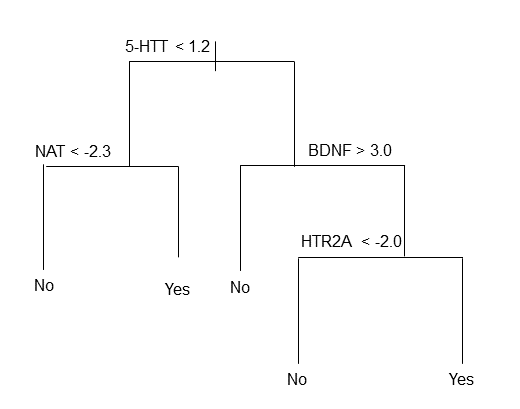
\includegraphics[width=12cm]{figures/decision_tree.png}
        \caption{A single decision tree in which drug-induced gene expression data are used to predict treatment effects}
        \label{fig:intr_tree}
      \end{figure}
      
      Figure \ref{fig:intr_tree} shows a single decision tree on fake drug expression data. In brief, for each time of splitting, we select a variable according to certain criteria and find a cutoff value of that variable to minimize the current loss. To grow a decision tree, the algorithm recursively splits the feature space of training data, and it stops when each leaf node has less than a minimum number of observations or the tree reaches the maximum depth. The \textit{Gini index}, a typical criterion used to make binary splits, measures the impurity of each node and is defined by \cite{james2013introduction}
      \begin{equation}
        G = \sum_{m=1}^T \sum_{k=1}^K  \hat{p_{mk}} (1 - \hat{p_{mk}}), 
      \end{equation}
      which measures total variance of binary classes for each leaf node. Here $T$ refers to the number of leaf nodes of a tree, $K$ denotes the number of classes, and $\hat{p_{mk}}$ represents the fraction of training observations in the mth region that are from the $k$th class. For binary classification $K$ is 2. 
      
      For tree-based regression, the procedure to grow a tree is similar to classification, but the criterion to make a binary split is different, which is \cite{james2013introduction}
      \begin{equation}
        \mathrm{EPE} = \sum_{m=1}^T \sum_{x_i \in r_m}  (y_i - \hat{y_{r_m}})^2, 
      \end{equation}

      Similarly, $T$ is the number of leaf nodes, $r_m$ is the $m$th leaf node, and $\hat{y_{r_m}}$ is the mean response of training observations in the $r_m$ region. Like linear models, penalty can also be imposed to reduce the complexity of tree to build models with lower variance. One form of regularization is to control the number of leaf nodes \cite{james2013introduction}:
      \begin{equation}
        G = \sum_{m=1}^T \sum_{k=1}^K \hat{p_{mk}} (1 - \hat{p_{mk}}) + \alpha T
      \end{equation}

      Note that in regression the average output of training observations falling into a leaf node can be regarded as the predicted value; in classification the probability of a class is estimated by the fraction of observations belonging to the class in the leaf node. 
      
      A single decision tree usually suffers from high variance which leads to poor predictive performance. Also, some observations may be predicted worse than others. To alleviate the problems of predicting with a single tree, “combining” many trees trained on different subsets of training data might improve predictive performances.Bagging, random forest, and boosting are powerful tools using this idea.
      
      Bagging, or bootstrap aggregation, is a procedure to reduce the variance of tree-based methods by averaging estimations from models trained on a number of training sets sampled by bootstrap. Observations are drawn with replacement in a bootstrap procedure. The prediction from bagging (for regression) is given by \cite{james2013introduction}
      \begin{equation}
        \hat{f}_{bag} (x) = \frac{1}{B} \sum_{b=1}^B \hat{f^{*b}}(x)
      \end{equation}
      where $B$ is the number of trees ensembled. For qualitative outputs, a majority vote can be taken to determine the predicted classes, i.e., the most commonly occurring class among the $B$ estimators for each observation.

      Random forest (RF) may be considered as a modified version of standard bagging. In random forest, only a subset of features is considered at each candidate split. Usually, features chosen for splitting are a minority of total features, and typically $m \approx \sqrt{p}$ (where p is the total number of features) is chosen in practice \cite{james2013introduction}. This aims to reduce the correlation between different trees, as aggregating many uncorrelated trees will benefit from a larger variance reduction than aggregating trees that are highly correlated.

      Gradient boosting is a general ML approach which aims at combining weak learners to produce an improved prediction model and is most often applied to decision trees \cite{friedman2001greedy}. Unlike bagging and random forest, boosting grows trees sequentially. In essence the algorithm tries to improve the model sequentially via fitting a learner to the residuals (or pseudo-residuals) from the previous model. Boosting for classification tree was first proposed by Freund and Schapire in \cite{freund1995desicion}, based on the idea of growing new trees by emphasizing more on observations poorly learned by previous trees. Friedman later developed a more general framework for boosting \cite{friedman2001greedy}.

      There are several advantages for tree-based methods. Firstly, decision tree mimics human decision processes and is relatively easy to interpret. For ensemble models, feature importance may be assessed by various means, for example improvement in the criterion for split (e.g., Gini index) and permutation importance in random forest, and the number of times a feature is used or total gain of splits using the particular feature in boosted trees. Also, tree-based models can handle qualitative and quantitative features and response with ease. In linear models, dummy variables are needed to handle qualitative features, but tree-based methods can absorb qualitative variable directly. Tree-based methods are also robust to outliers and model complex nonlinear relationships well.

    \subsubsection{Support Vector Machine}
      Support vector machine (SVM) is a typical maximum margin classifier that aims to separate different classes with a large "gap" \cite{cortes1995support}. By using the "kernel trick", SVM can map feature space from low dimensions to high, even infinite, dimensions, which makes problems that cannot be solved in low dimensions solvable.
      
      Here we will discuss SVM for classification only. We first assume that the data $(X, Y)$ is linearly separable and $Y \in \{-1, 1\} ^n$. Intuitively, we can model this problem as follows:
      \begin{equation}
        \min_{\gamma, w, b} \frac{1}{2} w^T w, s.t. y_i (w^T x_i + b) > 1, i = 1, \cdots, m
      \end{equation}
      
      Here $w$ denotes coefficients, $b$ stands for the intercept, and $s.t.$ in the equation is abbreviation of "subject to". This is a typical convex problem with linear restrictions, and it can be solved using convex optimization techniques. In reality, linear separable data is very rare, and SVM can also adapt to inseparable cases with nonlinear decision boundary. The reformulated equation is as follows:
      \begin{equation}
        \begin{split}
          & \min_{\gamma, w, b} \frac{1}{2} w^T w + C \sum_{i=1}^m \xi_i \\
           s.t. & y_i (w^T \phi (x_i) + b) > 1 - \xi_i, \xi_i > 0, i = 1, \cdots, m
        \end{split}
      \end{equation}

      Here, $\phi(xi)$ maps features $x_i$ from low to higher dimensions to capture nonlinear relationships; $\xi_i$ are slack variables that allows some observations to be on the wrong side; and $C$ controls the penalty of relaxing the functional margin. Figure \ref{fig:intr_svm} shows a hypothetical classification problem in which two observations fall into wrong sides after the introduction of slack variables.
      
      \begin{figure}[h]
        \centering
        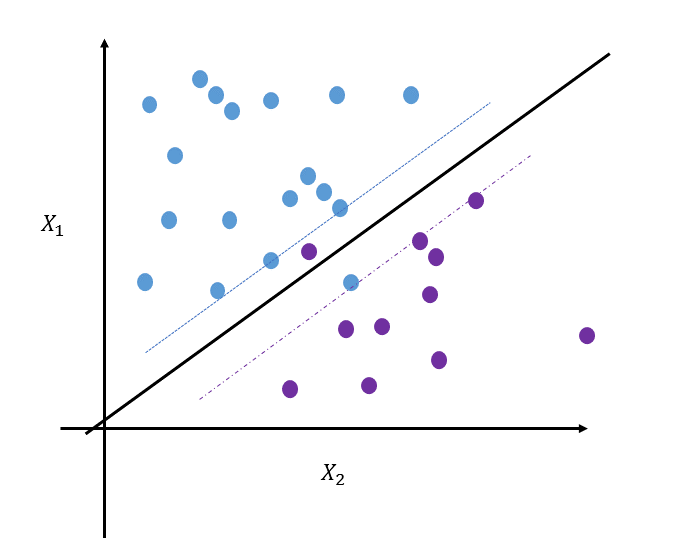
\includegraphics[width=10cm]{figures/SVM.png}
        \caption{A hypothetical classification task using linear SVM. Two observations fall into the wrong sides after the introduction of slack variables}
        \label{fig:intr_svm}
      \end{figure}

      The form of decision boundary can be transformed into the sum of inner product of feature mapped with the form of $\sum_{i=1}^m \alpha_i y_i \langle \phi(x_i), \phi(x) \rangle$, and $\langle \phi(x_i), \phi(x) \rangle$ is a kernel that measures the similarity between xi and x. The Gaussian (or radial basis function, RBF) kernel is one of the most widely used kernels to produce complex nonlinear decision boundaries. The Gaussian kernel can be expressed as: 
      \begin{equation}
        K(x, z) = \exp \bigg( - \frac{||x-z||^2}{2 \sigma^2} \bigg)
      \end{equation}

      There are serval key characteristics of SVM. First, the decision boundary of SVM is actually determined by observations near the boundary, and thus data points far away from the boundary have little effect on the decision boundary. It models nonlinear relationships well, and various kernels can be applied to make different complex decision boundaries to satisfy different classification problems \cite{bishop2006pattern}.

      SVM has been employed for drug or target discovery in earlier studies. For example, in a recent work, the authors integrated several layers of drug properties including chemical structures and proximity of targets in an interaction network and expression profiles and used SVM to predict therapeutic classes \cite{napolitano2013drug}. Another study adopted SVM trained on molecular structure, molecular activity, and phenotype data to discover new indications for drugs \cite{wang2013drug}. A study we mentioned earlier \cite{aerts2007pharmacological} employed SVM and DNN to learn drug therapeutic categories from gene expression data. Regarding the application of SVM on drug target discovery, studies \cite{bakheet2009properties,li2007prediction} utilized SVM on structural or chemical properties of known drug targets to identify promising drug targets.

      In our recent application, we used SVM with Gaussian kernel and found SVM in general performed favorably compared to other methods \cite{zhao2018drug}. We used the Python package "scikit-learn" \cite{pedregosa2011scikit,buitinck2013api} for implementation, but similar packages in R or other programming languages are also available.

      Regarding the limitations of this approach, SVM models are often difficult to interpret, and there is a lack of widely used criteria to quantify the importance of individual features. In the case of drug repositioning or target discovery, this may be a limitation given that we are usually interested in identifying which genetic or biological factors contribute to the treatment effects on diseases. As a kernel-based method, drug repositioning with SVM employs a comparable principle to other "similarity-based" approaches (e.g., a drug $X$ with high similarity to a known treatment A may also be able to treat the same disease) \cite{hodos2016silico}. Similarly, perturbation of a gene may induce a pattern of expression profile that is similar to that of a drug, then compounds acting on the gene may have similar mechanisms to the drug. Thus, one limitation is that such an approach may not be very good at revealing candidates with novel mechanisms of actions \cite{hodos2016silico}.

    \subsubsection{Deep Neural Networks}
      Deep learning has attracted increasing attention in recent years and contributed to significant advances in many fields such as computer vision. Deep neural networks (DNN) are based on the concept of  "representation learning" \cite{bengio2013representation} and are very good at capturing nonlinear relationships. Many different network architectures have been developed, but here we only discussed feedforward neural networks with fully connected layers.

      By using multiple hidden layers, DNN can handle more complex relationships than a simple single-layered network. The optimal number of hidden layers and neurons will depend on the nature and complexity of the problem as well as the data size. DNN usually requires relatively large sample sizes to achieve good predictive power as the number of parameters is large and overfitting can be a major problem. Dropout is a simple and widely used approach to avoid overfitting by “inactivating” a proportion of neurons randomly during training \cite{srivastava2014dropout}. Feature selection and shrinkage can also be applied by employing L1 and L2 regularization \cite{zou2005regularization}. There are also numerous other hyper-parameters to choose from, such as the activation function, learning rate, momentum, batch size, etc. For activation function of hidden layers, ReLU is often used. In the output layer, sigmoid function can be used in binary classification problems and softmax in multi-classification problems. The performance of DNN is promising in recent studies of drug repositioning and drug category classification \cite{aliper2016deep,zhao2018drug}. Nevertheless, DNN models are hard to interpret, and the choice of hyper-parameters is often difficult. The computational and time costs for training a model are relatively high (especially for large datasets); however, the use of graphic processing units (GPUs) can greatly accelerate the computing speed.

      With the rapid development of deep learning methodologies, they have been increasingly used for drug repurposing \cite{aliper2016deep,zhao2018drug,xie2017discovery} or prediction of various drug properties or toxicities. For example, Klambauer et al. applied deep neural networks on chemical features of compounds to predict their toxicities \cite{mayr2016deeptox}. Ryu et al. employed deep learning to improve prediction of drug-drug and drug-food interactions \cite{ryu2018deep}. Deep learning has also been used to predict synergistic effects of drugs in cancer therapy \cite{preuer2018deepsynergy}. Readers may also refer to recent reviews on the applications of deep learning in biomedicine and drug discovery \cite{baskin2016renaissance, chen2018rise, ching2018opportunities}.

    \subsubsection{Cross Validation to Assess Predictive Performance}
      Above we have introduced several common ML algorithms for training a prediction model. Meanwhile, assessing the performance of model is a critical issue, and the performance of the model in train set can dramatically underestimate of the true prediction error.
    
      To avoid overoptimistic estimation of model performance, the prediction error can be estimated in a new dataset independent of the training set, if such data is available. However, data is often limited, and a more popular approach is K-fold cross validation. A typical practice is to firstly split the entire dataset into K folds evenly and then set side onefold of data as testing set and train on the other folds in each loop. There is no fixed rule to determine K, but it is often set at 5 or 10. A very low K (e.g., leave-one-out cross validation) will lead to almost unbiased but high variance of the prediction error estimate, as the training sets are highly similar. Increasing K will reduce the variance but may increase the bias \cite{friedman2001elements}.
      
      In practice, one often needs to tune hyper-parameters, and dividing the data into training and testing sets will not be sufficient. In some studies, the authors would train the model in the training set and pick the hyper-parameters that give the best predictive performance in test set and then report the corresponding prediction error. (In case of cross validation, the "best" prediction error may be averaged over the K folds). However, such an approach still tends to give overoptimistic estimates of the prediction error as one is picking the best-performing parameters each time which may not be generalized to a completely new dataset \cite{varma2006bias}. To avoid this problem, the testing set should not be involved in parameter tuning. For example, the dataset can be divided into training, validation, and testing sets, in which the hyper-parameters are chosen based on predictive performance in the validation set. A more advanced approach is nested K-fold cross validation \cite{varma2006bias}. In this case, inner K-fold cross validation is used to choose the best hyper-parameters, and the performance of the model with the best parameters chosen is evaluated on the testing set.

    \subsubsection{Criteria for Model Selection}
      Here we describe criteria for assessing model fit and predictive performance. For regression, the most commonly used criteria are mean squared error loss. Below we discuss the metrics for classification.

      Log loss, or cross entropy, measures the negative log-transformed probability of belonging to expected class for each observation. Its equation is
      \begin{equation}
        \mathrm{EPE} = - \sum_i y_i \log p(x_i) + (1 - y_i) \log (1 - p(x_i)).
      \end{equation}
      Therefore, the higher the probability an observation belongs to the expected class, the smaller the log loss value of the observation. Cross entropy is a widely used objective function in classification tasks.

      If there is a predefined specific threshold to define a positive or negative outcome (e.g., say it is generally agreed that predicted probability $> 30$\% represents positive outcome), different measures such as sensitivity (aka recall), specificity, precision (aka positive predictive value), and F1 score (harmonic mean of precision and sensitivity) can be computed accordingly. However, often we may not have such a predefined threshold, and we may wish to consider the overall performance of the model under a variety of possible thresholds. In this case we may use the area under the receiver operating characteristic (ROC) curve (AUROC) or area under the precision-recall curve (AUPRC) as metrics of predictive performance.
      
      The ROC curve records the true positive rate (sensitivity) against false positive rate (1- specificity) at different thresholds. Area under the ROC curve (AUROC) is a commonly used metric to assess predictive performance especially in the medical field. For problems with class imbalance, it has been argued that AUPRC may better reflect the model performance \cite{davis2006relationship}.

    \subsubsection{Common Issues of Machine Learning in Biomedical Studies}
      Overfitting refers to overlearning of a model on the training data, leading to poor performance when applied in a new situation. Underfitting describes an opposite phenomenon, in which the model fails to capture the complex relationships within the data. A closely related concept is the “bias-variance” tradeoff. In general, models that are complex will have small bias but higher variance, while simpler models enjoy lower variance but have increased bias. Several approaches may be employed to reduce the risk of overfitting. For example, one may reduce the number of features by preselection or some form of dimension reduction, apply heavier regularization penalty to make the model simpler, or switch to less complex ML models. If possible, obtaining larger sample sizes will also alleviate the problem. Underfitting can be overcome by opposite strategies. 
      
      However, how do we know whether a model overfits or underfits in practice? A typical strategy is to examine or plot a curve of the training and testing errors. If training error is unacceptably high and the gap between the two errors is small, then the complexity of the model chosen may be too low, or underfitting is present. If the training error is close to 0 but testing error is high, the model might be overfitting.

      Imbalanced data is a problem often encountered in biomedical applications in which observations with positive outcome may be uncommon. For example, only a few people may develop a disease or complication, or only a minority of the drugs can treat a specific disorder. There are several common strategies for imbalanced data, such as down-sampling the majority class, up-sampling of the minority class, and constructing new cases by methods such as SMOTE \cite{chawla2002smote}. Here we briefly describe how to tackle this problem with class weights. If the default weight for each observation is 1 and positive observations are rare, the total weights of positive and negative observations will be imbalanced. To remedy the situation, we can \textit{increase} the weight for each positive observation to balance the total weights of the positive and negative classes. This strategy can also be used in multi-class classification problems. In a recent work of drug repositioning, we did observe obvious improvement in predictive power using the above weighting scheme \cite{zhao2018drug}.

  \section{Machine Learning Methods for ITE Estimation}
    Machine learning is a data-driven approach, without strong modeling assumptions, and techniques such as cross validation and various penalties can be incorporated to avoid overfitting, reducing the possibility of false discovery. There is also a rise in the number of studies using machine learning approach to estimate ITE. typically, there are two typical steps in estimation of heterogeneous treatment effects. We need to identify groups of heterogeneity in treatment effects firstly, and then to estimate of individual treatment effects, ie, individual risk prediction \cite{scarpa2019assessment}. The are mainly two streams in application of machine learning approaches to ITE estimation: averaged treatment effect of subgroups defined by learning algorithms and ensembled approaches based on tree-based methods.
    
    Some of recent studies focus on detecting subgroups of heterogeneity in treatment effects. Specifically, these studies try to to estimate the difference of averaged outcome between treatments and controls in pre-specified subgroups \cite{gail1985testing} or subgroup defined by learning algorithms \cite{su2009subgroup, su2011interaction, athey2016recursive,foster2011subgroup, lipkovich2011subgroup}. Su et. al. employed interaction tree to iteratively searching subgroups based on treatment effect \cite{su2009subgroup,su2011interaction}. Similarly, causal trees proposed by Athey and Imbens estimate the treatment effect at the leaves of the tree \cite{athey2016recursive}. However, the definition of subgroup is arbitrary and somewhat algorithm dependent, the generality of subgroup algorithms maybe poor, and these subgroup algorithms tend to over-estimate the heterogeneity present. As stated in the study \cite{wager2018estimation}, the impediment of iteratively searching for subgroups present obvious treatment effect and reporting only the results for subgroups with extreme treatment effects to highlight heterogeneity may be highly spurious. In the high dimensional setting, it's still very challenging to divide subjects into appropriate subgroups \cite{powers2017some}. It's the same case for genomic data. 

    Forests-based methods have gained popularity in ITE estimation in the past years \cite{wager2018estimation,kunzel2019metalearners,lu2018estimating,dasgupta2014risk,hill2013assessing,hill2013assessing,green2012modeling}, because forests-based methods have very nice features. Most importantly, they have excellent interpretability since variables contributing to prediction can be extracted, and even can visualize the procedure of decision-making by plotting some important trees. Forests-based methods capture complex interactions in data. A study shows that forests-based methods can discover predictive and stable high-order interactions \cite{basu2018iterative}. They also has other benefits, like less likely to overfit and robust to missing values. Studies \cite{green2012modeling,hill2011bayesian, hill2013assessing} employs bayesian forest-based methods to estimate heterogeneous treatment effects, which are based on Bayesian additive regression tree (BART) method \cite{chipman2010bart}. One advantage of this kind of approach is that reliable intervals for treatment effects can be readily obtained by MCMC sampling. Some other methods in frequentist form, like Meta learners and deep learning based, for ITE estimation could be found in \cite{kunzel2019metalearners,johansson2016learning,powers2017some}. Powers et al. proposed causal boosting, causal Multivariate adaptive regression splines (MARS) and pollinated transformed outcome (PTO) forests to fit adjusted outcomes \cite{powers2017some}. Another study employed deep learning to make counterfactual inference on ITE \cite{johansson2016learning}. In practice, these approaches try to fit $\mu_1(\mathbf{x})$ and $\mu_0(\mathbf{x})$ simultaneously / separately and estimate the difference by computing the different between $\mu(\mathbf{x},w)$ and $\mu(\mathbf{x}, 1-w)$.  Similarly, metaalgorithms decompose estimation of the CATE into several sub-regression tasks, that can be tackled with any supervised learning method \cite{kunzel2019metalearners}. A limitation of these studies is lack of formal statistical inference results \cite{wager2018estimation}. Wager et al. proposed causal forests with honest to estimate ITE \cite{wager2018estimation}. In causal forests with honest, training set is splited into two parts, one partition is used for tree growing, and the other partition is utilized to make honest estimation; Moreover, the authors have showed that causal forests with honest have good asymptotic properties \cite{wager2018estimation}.
  
  \section{Summary}
    In this section, we introduced the current situation of drug development and difficulties in the process of developing a new medication, reviewed some studies using computational approaches to drug target discovery and purposing, and discussed their limitations. As the technique behind the computational method largely belongs to the field of machine learning, we gave a detailed introduction of machine learning approaches, with some biomedical applications of corresponding ML methods as examples. Then we went into a more clinically relevant topic of discovering ITE. For estimation of ITE, we focused on methods discovering ITE using machine learning based approaches, reviewed some relevant studies based on ML approaches, and pointed out possible limitations of these studies.
     
\chapterend